\subsection{\name: From Paths to Configurations}
\todo{Motivate about OSPF synthesis} \\


In \Cref{fig:bgpeg}, we show how \name configures BGP in domain AS0 
to ensure that traffic from $src$ to $dst$ is routed across domains 
such that it follows the path $p$ provided as input. Suppose path (1) is
provided as input. G3 receives a route for $dst$ with AS path length 1
(AS2), while G1 and G2 will receive a route for $dst$ with 
AS path length 2 (AS1, AS2). Since, we need to send traffic along
G3, we do not need to configure any additional BGP variable for $dst$;
\Cref{alg:bgppathrules} will choose the best route for $dst$ 
via G3 (which is the gateway of the input path) as all routes have
the same local preference (0) and AS path length is used to  and $R1$ will
send the packet to $dst$ to G3 along the shortest path (which 
follows the subpath of $p$ from $R1$ to $G3$ by OSPF synthesis). 

Consider the example of input path (2) for $src$ to $dst$ 
in \Cref{fig:bgpeg}. Since, $G1$'s route has a longer AS 
path length greater than $G3$'s route and equal to $G2$'s route,
we need to set the local preference of route received by $G1$ 
(from $G4$) to 100 (any positive value). Thus, \Cref{alg:bgppathrules} 
will select $G1$ as the exit gateway for $dst$. The subpath
$R1$ to $G1$ will be given appropriate weights by the OSPF
synthesis phase so that the synthesizing configurations 
forward traffic along the input path. 

Case 3: Multiple gateways, done using iBGP filters. 
\begin{figure}[!t] 
	\centering
	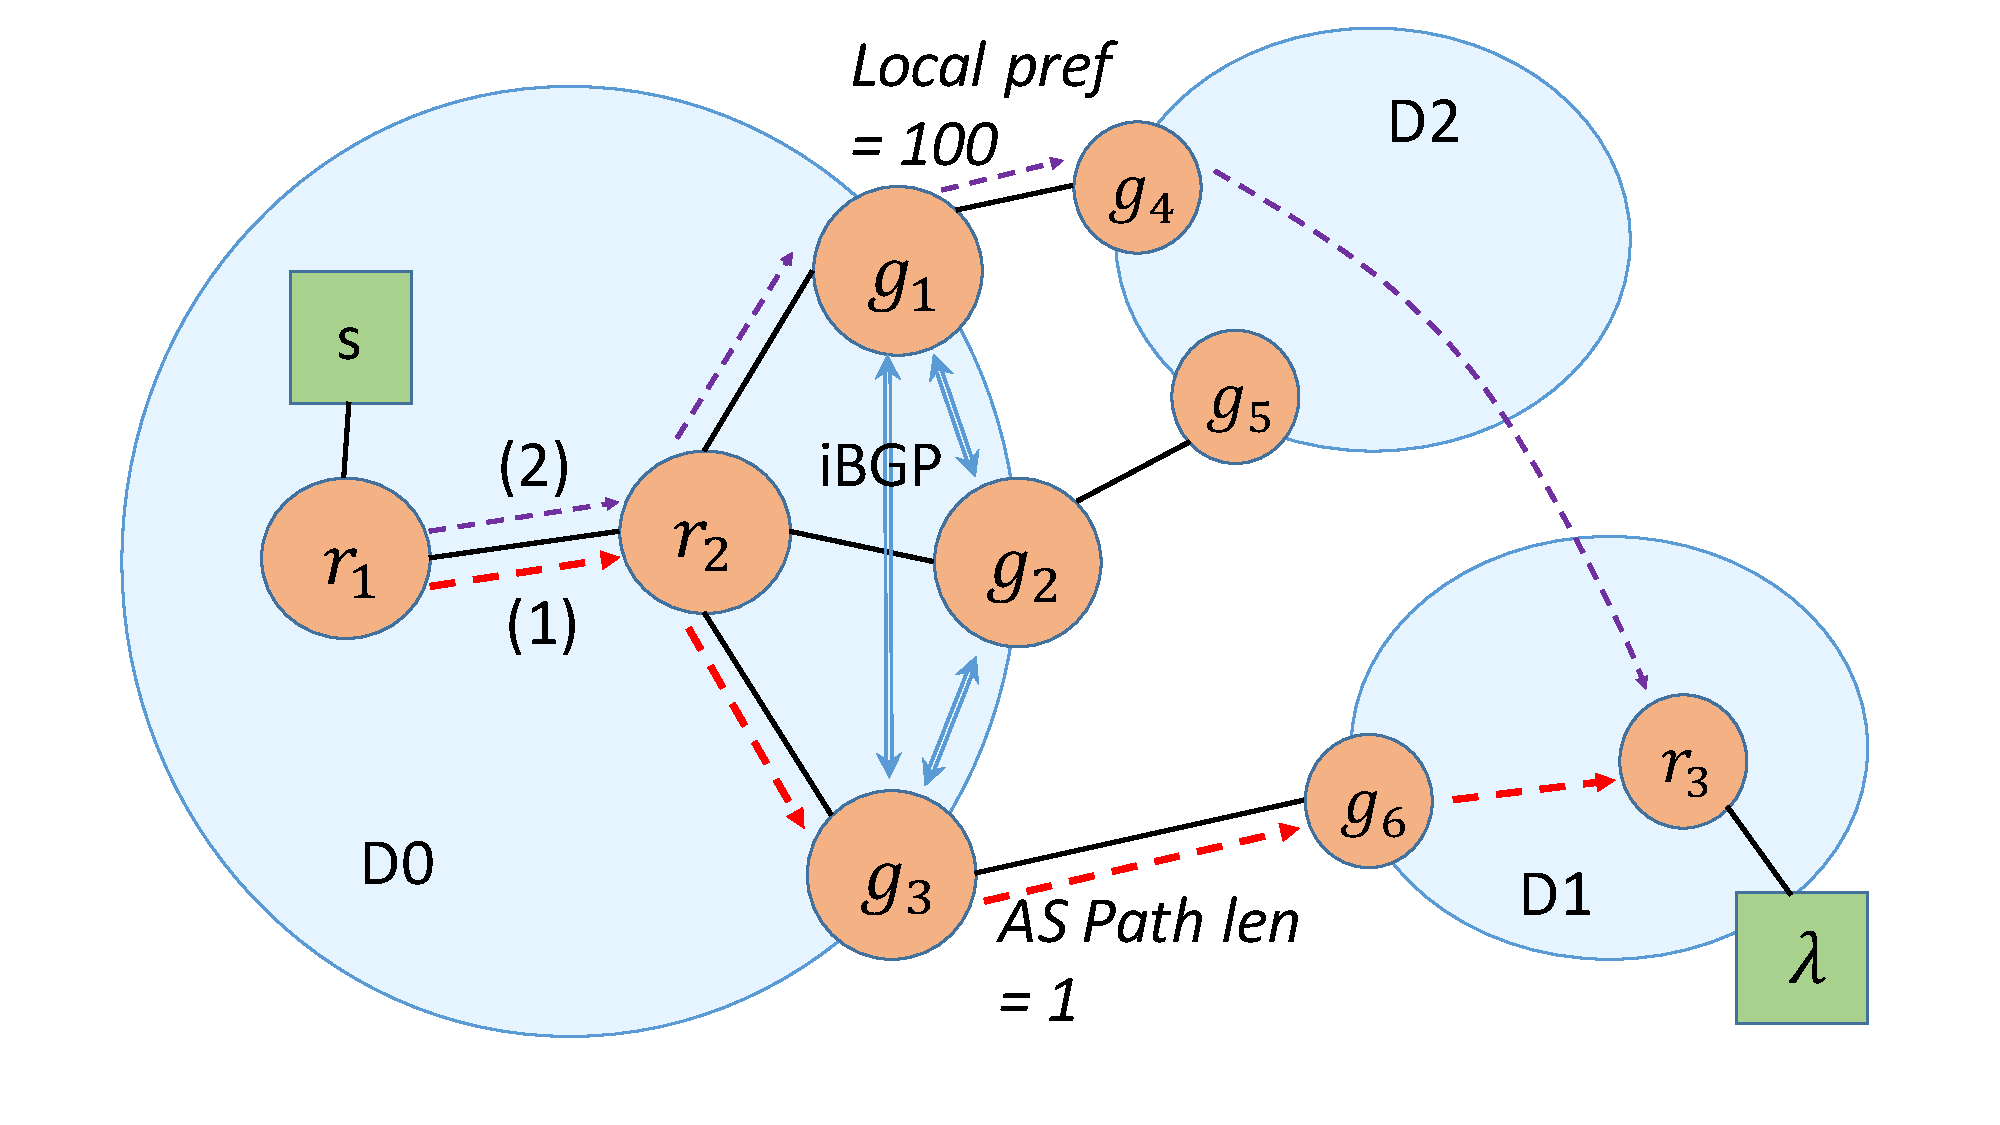
\includegraphics[width=\columnwidth]{figures/bgp-example.pdf}
	\caption{Example} \label{fig:bgpeg}
\end{figure}


\section{Background}
\subsection{OSPF}

\subsection{BGP}
BGP is a path-vector routing protocol that connects 
different autonomous systems (ASes), where each AS
comprises of one or more routers (typically managed
by a single entity). 

\minisection{eBGP}
\\
\minisection{iBGP}
Multiple routes received to a dst from domain
iBGP synchs these routes among different routers
and chooses the best route according to \Cref{alg:bgppathrules}.

\minisection{Route Redistribution}
Main point is that routers only redistribute
eBGP routes (and not iBGP routes) into OSPF.
\name uses this to enforce the particular
BGP gateway

\subsection{BGP Best Path Selection Algorithm}
A BGP router receives multiple paths to the destination: (1)
external routes from border routers of neighbouring domains using
eBGP, and (2) routes learned by other BGP routers 
of the domain which are advertised using iBGP. 
BGP decides the best path to install in the 
forwarding table based on different metrics like local preferences,
AS path lengths and type of routes~\cite{bgp}. BGP uses \Cref{alg:bgppathrules}\footnote{
The actual BGP implementation has several other criteria
for choosing best routes, the configurations synthesized
by \name will use the abridged algorithm (which considers
the rules in relative ordering to actual BGP). 
} 
to select the best route 
from the set of received announcements from eBGP 
and iBGP (after applying the configured route filters). 
\begin{algorithm}
	\begin{footnotesize}
		\caption{BGP Best Path Algorithm}
		\label{alg:bgppathrules}
		\begin{algorithmic}[1]
			\State{[Input] $R \leftarrow$ eBGP and iBGP routes for $dst$} 
			\State{[Output] $r_{best}$ : Best BGP route} \newline \newline
			/* Find routes with highest \emph{local preference} */
			\State{$R_{lp} = \{r \in R ~| ~\forall r_1 \in R. ~r.local\_pref \geq r1.local\_pref\}$}
			\If{$|R_{lp}| = 1$}
			\State{$r_{best} = r \in R_{lp}$}
			\Else \newline
			\indent /* Prefer the path with the smallest \emph{AS Path length} */
			\State{$R_{as} = \{r \in R_{lp}  ~|~ \forall r_1 \in R_{lp}. ~r.path\_len \geq r_1.path\_len\} $}
			\If{$|R_{as}| = 1$}
			\State{$r_{best} = r \in R_{as}$}	
			\EndIf
			\EndIf
%				\State{ . }
%				\State{Prefer the path with the lowest \emph{multi-exit discriminator} (MED).}
%				\State{Prefer eBGP over iBGP paths.}
%				\State{Prefer the route that comes from the BGP router with the lowest \emph{router ID}.}
		\end{algorithmic}
	\end{footnotesize}
\end{algorithm}

